\documentclass{standalone}
\usepackage{tikz}
\usepackage{xcolor}
\usetikzlibrary{arrows, arrows.meta, backgrounds}
\pagestyle{empty}

\begin{document}
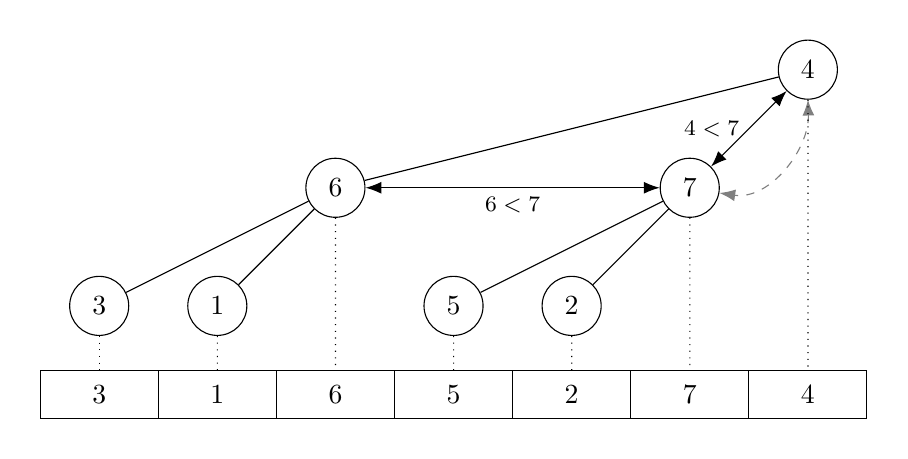
\begin{tikzpicture}[scale=1.5,elem/.style={draw,shape=circle,minimum size=0.75cm},background rectangle/.style={fill=white},show background rectangle]

% Draw the poplar heap nodes
\node[elem] (n1) at (0,0) {3};
\node[elem] (n2) at (1,0) {1};
\node[elem] (n3) at (2,1) {6};
\node[elem] (n4) at (3,0) {5};
\node[elem] (n5) at (4,0) {2};
\node[elem] (n6) at (5,1) {7};
\node[elem] (n7) at (6,2) {4};

% Links between the nodes
\draw[{Latex[length=2mm]}-{Latex[length=2mm]},bend left] (n7) -- (n6) node[midway,left,font=\footnotesize] {$4 < 7$};
\draw[dashed,{Latex[length=2mm]}-{Latex[length=2mm]},bend left,draw=gray] (n7) to[out=45,in=125] (n6);
\draw[{Latex[length=2mm]}-{Latex[length=2mm]}] (n3) -- (n6) node[midway,below,font=\footnotesize] {$6 < 7$};
\draw (n7) -- (n3);
\draw (n6) -- (n5);
\draw (n6) -- (n4);
\draw (n3) -- (n2);
\draw (n3) -- (n1);

% Draw the array representation of the poplar heap 
\tikzstyle{every node}=[draw,shape=rectangle,minimum width=1.5cm,minimum height=0.6cm,anchor=center];
\foreach \x [count=\idx] in {3,1,6,5,2,7,4}
  \node (r\idx) at (\idx-1,-0.75){\x};

% Explicitly link the nodes to the array representation
\foreach \x in {1,...,7}
   \draw[dotted] (n\x) -- (r\x);

\end{tikzpicture}
\end{document}
